\documentclass[UTF8,a4paper,11pt]{ctexart}

\usepackage{amsmath}
\usepackage{booktabs}
\usepackage{geometry}
\usepackage{graphicx}
\usepackage{hyperref}
\usepackage{xcolor}
\usepackage{listings}

\geometry{margin=2.4cm}
\graphicspath{{../result/}{result/}}
\hypersetup{
  colorlinks=true,
  linkcolor=blue,
  urlcolor=blue,
  citecolor=blue
}

\lstdefinestyle{trace}{
  basicstyle=\ttfamily\small,
  breaklines=true,
  frame=single,
  columns=fullflexible,
  backgroundcolor=\color{gray!6}
}

\title{可验证符号算术轨迹的从零监督训练：\\一个小型 Transformer 的初步实验}
\author{Primordial Disjunction}
\date{\today}

\begin{document}
\maketitle

\begin{abstract}
本文研究一个可控的符号算术生成任务：给定前缀表达式，模型需要生成显式逐步计算轨迹，并输出最终十进制数值。该实验的长期动机是考察 Transformer 是否能够在符号表达式空间和数值空间之间建立可验证的映射，进而为后续的反向符号搜索、beam search verifier 和强化学习式奖励优化提供基础。当前实现训练了一个从零开始的小型 Qwen 风格因果语言模型，仅使用无限在线生成的 \texttt{forward} 数据。实验结果显示，在四类浅层算术模板上，模型训练 loss 已降至 $10^{-5}$ 量级，训练内置周期评测在后期连续达到 \texttt{forward} exact match 和 numeric success 均为 1.0；可视化样例中，模型能够逐 token 复现加法、带负数减法以及进位/借位 trace。与此同时，当前评测样本量较小，尚未验证深度外推、反向索引或 RLHF/RLAIF 设置，因此结论应视为一个可运行的初步正结果，而不是完整的泛化证明。
\end{abstract}

\section{问题设定}

原始设想是构造一个可验证的符号搜索任务：
\[
  v \mapsto e,\qquad \mathrm{eval}(e) \approx v,
\]
例如从 \texttt{3.14626} 反推出 \texttt{add(sqrt(2),sqrt(3))}。这类任务像一个从连续数值到离散语法结构的近似反向索引：若模型成功，它可能学到某种可组合的 hash inverse；若失败，则说明类似 bloom-filter 的记忆机制在符号外推上可能很弱。

当前代码库优先实现并训练了前向可验证任务：
\[
  e \mapsto (T(e), \mathrm{eval}(e)),
\]
其中 $e$ 是表达式，$T(e)$ 是逐步计算 trace。输入为
\[
  \texttt{|forward|} + \mathrm{tokens}(e),
\]
输出为
\[
  \texttt{|beginOfThink|} + T(e) + \texttt{|endOfThink|} + \mathrm{render}(\mathrm{eval}(e)).
\]

\section{数据生成}

表达式由 \texttt{data\_generate.py} 在线采样。当前激活的 \texttt{forward} 模板如下：

\begin{lstlisting}[style=trace]
add leaf leaf
mul leaf leaf
add neg leaf leaf
add leaf neg leaf
\end{lstlisting}

叶子常数范围为 $[1,500]$，十进制输出保留 5 位小数。对于 \texttt{add}、\texttt{mul}、\texttt{neg} 以及由负数加法诱导出的 \texttt{sub}，生成器会写出结构展开和具体竖式步骤。例如加法 trace 会包含：

\begin{lstlisting}[style=trace]
r0 = add r1 r2
r1 = 108
r2 = 107
r0 = add 108 107
    add 108 107
    = addPad 108 107
    = addPos (8 7) (0 0) (1 1)
    = addPosRes (5 1) (0 0) (2 0)
    = addRes 5 (1 0) (0 2) 0
    = addRes 5 1 2 0
    = 0215
    = 215
r0 = 215
\end{lstlisting}

这样设计的好处是，目标不是黑箱回归一个数字，而是学习一个可检查的算法轨迹。若未来加入 verifier，可以分别检查语法合法性、每一行局部计算和最终数值误差。

\section{模型与训练}

模型为从零训练的 Qwen 风格 decoder-only Transformer。词表由任务 token、运算符、数字、标点和 trace token 组成，而不是复用自然语言 tokenizer。主要配置见表 \ref{tab:model}。

\begin{table}[h]
\centering
\begin{tabular}{lr}
\toprule
配置项 & 数值 \\
\midrule
词表大小 & 42 \\
参数量 & 10,450,304 \\
层数 & 24 \\
hidden dim & 128 \\
attention heads & 8 \\
KV heads & 2 \\
head dim & 64 \\
max sequence length & 2304 \\
batch size & 4 \\
learning rate & $3\times 10^{-4}$ \\
weight decay & 0.01 \\
\bottomrule
\end{tabular}
\caption{当前实验使用的模型与训练配置。}
\label{tab:model}
\end{table}

训练采用标准 next-token SFT。prompt 部分 label 置为 \texttt{-100}，只在输出 trace 和最终答案上计算交叉熵。训练任务当前仅启用 \texttt{forward}，因此 \texttt{inverse} 和 \texttt{simplify} 的结果不应纳入模型能力结论。

\section{实验结果}

当前训练日志包含 40,382 条 loss 记录，最后记录步数为 118,565，最后 loss 为 $1.91\times10^{-5}$，日志中最小 loss 为 $2.95\times10^{-6}$。内置评测日志在后期每 1000 step 对 2 个 \texttt{forward} 样本评测一次；从 109,000 到 118,000 step 的最近 10 次评测中，\texttt{forward} exact match rate 和 numeric success rate 均为 1.0，invalid rate 为 0.0。

\begin{table}[h]
\centering
\begin{tabular}{lccc}
\toprule
阶段 & exact match & numeric success & invalid \\
\midrule
step 109000--118000 的周期评测 & 1.0 & 1.0 & 0.0 \\
step 118000 可视化样例 & 1.0 & 1.0 & 0.0 \\
\bottomrule
\end{tabular}
\caption{当前日志中的 \texttt{forward} 初步结果。周期评测每次仅 2 个样本，因此该表说明训练已收敛到可用状态，但不能单独证明大样本泛化。}
\label{tab:results}
\end{table}

\begin{figure}[h]
\centering
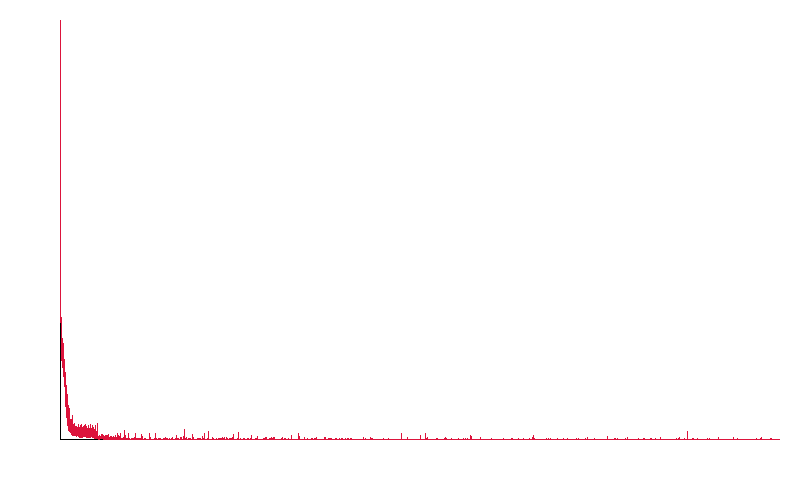
\includegraphics[width=0.9\linewidth]{loss.png}
\caption{训练过程保存的 loss 曲线。该图由当前代码库的简易 PNG writer 生成。}
\label{fig:loss}
\end{figure}

从 \texttt{result/visual.txt} 看，模型在 step 118000 对两个可视化样例均逐 token 完全匹配。第一个样例是 \texttt{add(108,107)}，模型正确生成进位步骤并输出 \texttt{215.00000}。第二个样例是 \texttt{add(384,neg(416))}，模型将其规约为 \texttt{sub(384,416)}，再翻转为带负号的 \texttt{sub(416,384)}，正确处理借位并输出 \texttt{-32.00000}。

\section{结果怎么看}

这个结果是一个清楚的工程正信号：数据格式、tokenizer、长 trace 监督、模型结构和训练循环都已经打通，小模型确实能够学会当前模板分布内的显式算术轨迹。尤其是带负数的样例说明模型不只是输出最终数字，也能复现由生成器规定的中间规约形式。

但从研究结论上还要谨慎。当前 \texttt{forward} 样本空间估计为 $10^6$，模板只有 4 个，且评测样本数很小；模型很可能已经在这个受限分布上形成了强模式拟合。原始课题中最有趣的部分，即数值到表达式的反向搜索、深度外推、不同进制比较、beam verifier 和 RLHF/RLAIF 奖励，目前还没有形成实验证据。

\section{下一步实验}

下一步建议优先补齐三件事。第一，增加独立大样本评测脚本，至少对 \texttt{forward} 采样 1,000--10,000 个样本，报告 exact match、numeric success、invalid rate 和按模板分组的错误率。第二，将模板从一层算术扩展到混合表达式，并做 depth split：训练 depth $\leq 3$，测试 depth $=4,5,6$。第三，重新启用 \texttt{inverse}，先用 beam search + verifier 做 top-$k$ success，再考虑基于
\[
  r(e,v)=-\log(|\mathrm{eval}(e)-v|+\epsilon)-\lambda |e|-\mathrm{invalid\ penalty}
\]
的强化学习或偏好优化。

\section{结论}

当前项目已经得到一个可信的第一阶段结果：从零训练的小型 Transformer 可以在受控模板上学习可验证的符号算术 trace，并在训练后期的小样本评测中达到完全匹配。这个结果值得作为论文的初步实验写入，但论文主张应限定为 ``forward trace learning works in a controlled setting''。要支撑更强的 ``反向符号搜索'' 或 ``bloom-filter-like 外推'' 论断，还需要系统的反向任务、深度外推和大样本评测。

\end{document}
